\documentclass[14pt]{beamer}

\usepackage[utf8x]{inputenc}
\usepackage[T1]{fontenc}
\usepackage[french]{babel}
\usepackage{float}
\usepackage{graphicx}
\usepackage{amsthm}

\fontfamily{verdana}

\definecolor{mybackground}{RGB}{29, 29, 29}
\definecolor{mytext}{RGB}{36, 187, 223}
\setbeamercolor{normal text}{bg=mybackground, fg=white}
\setbeamercolor{title}{fg=mytext}
\setbeamercolor{block title}{fg=mytext}
\setbeamerfont{title}{series=\bfseries}

\newenvironment{aquote}[1]{%
    \pushQED{#1}%
    \begin{quote}
}{%
    \newline
    \par\nointerlineskip\noindent\hfill \textcolor{mytext}{\popQED}%
    \end{quote}%
}

\title{The Online Filter Bubble}
\author{Alexandru Fikl}
\date{October 5, 1991}

\begin{document}

\begin{frame}
 \titlepage
\end{frame}

\begin{frame}
    \begin{aquote}{Mark Zuckerberg, Facebook}
        A squirrel dying in your front yard may be more relevant to your interests
        right now than people dying in Africa.
    \end{aquote}
\end{frame}

\begin{frame}
    \begin{figure}[h!]
    \centering
    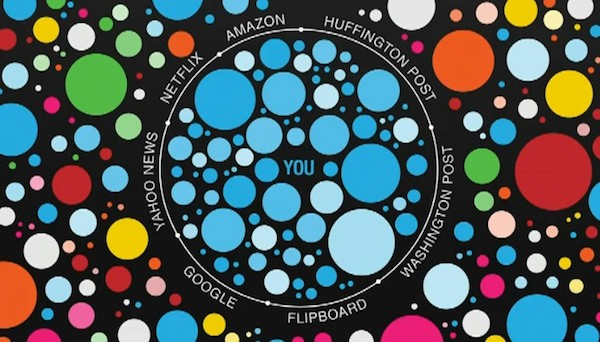
\includegraphics[scale=0.5]{./img/filter-bubbles.jpg}
    % filter-bubbles.jpg: 600x342 pixel, 72dpi, 21.17x12.06 cm, bb=0 0 600 342
\end{figure}
\end{frame}

\begin{frame}
    \begin{aquote}{Eric Schmidt, Google}
        It will be very hard for people to watch or consume something that has not
        in some sense been tailored for them.
    \end{aquote}
\end{frame}

\begin{frame}
    \begin{columns}[T]
    \begin{column}{.5\textwidth}
     \begin{block}{Adrian}

     \hbox{}

    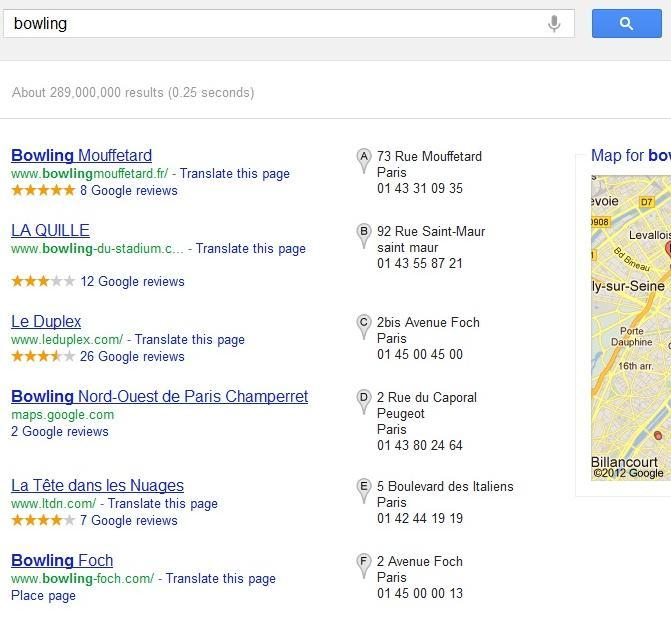
\includegraphics[scale=0.3]{./img/bowling.jpg}
    \end{block}
    \end{column}
    \begin{column}{.5\textwidth}
    \begin{block}{Me}
% Your image included here

    \hbox{}

    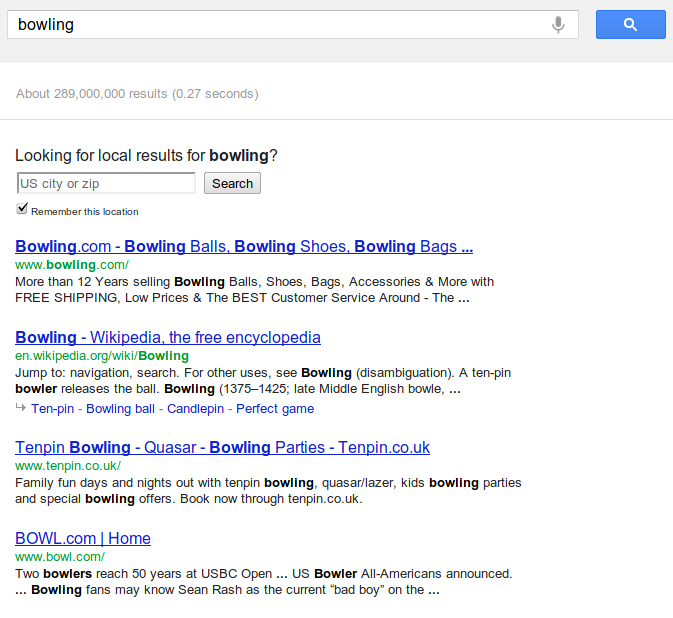
\includegraphics[scale=0.3]{./img/bowling.png}
    \end{block}
    \end{column}
  \end{columns}
\end{frame}

\begin{frame}
    \begin{figure}[h!]
    \centering
    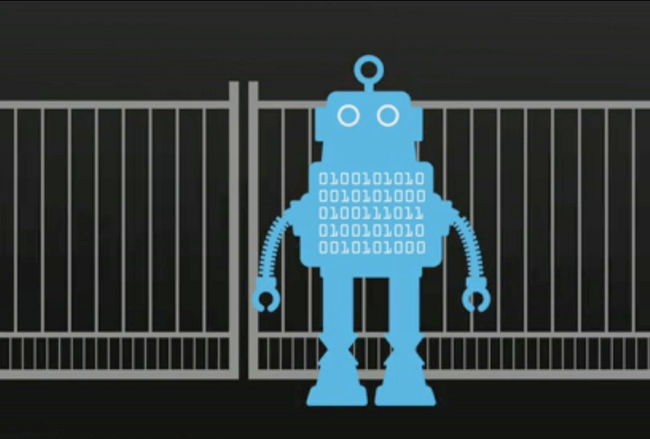
\includegraphics[scale=0.4]{./img/filter-bubbles2.jpg}
    % filter-bubbles2.png: 635x347 pixel, 96dpi, 16.80x9.18 cm, bb=0 0 476 260
\end{figure}
\end{frame}

\begin{frame}
\begin{figure}[h!]
    \centering
    
\includegraphics[scale=0.6]{./img/filter-bubbles3.jpg}
    % filter-bubbles3.jpg: 640x363 pixel, 96dpi, 16.93x9.60 cm, bb=0 0 480 272
\end{figure}
\end{frame}

\begin{frame}
\begin{center}
    {\Large Thank you for your attention!}

    \vfill
    {\huge Questions!?}
    \vfill
    \small Credits to \textbf{Eli Pariser, www.ted.com, the internet}.
\end{center}
\end{frame}

\end{document}